\documentclass[,a4paper,12pt,french]{article}

\usepackage{../../Style}

\pagestyle{empty}

%\renewcommand\tabularxcolumn[1]{m{#1}}

\newcommand{\\vva}{
\begin{center}
\begin{tabularx}{\linewidth}{|X|X|} \hline
\Centering{
\begin{tikzpicture}[scale=1]
\begin{axis}[
axis x line=bottom,
axis y line = left,
axis lines=middle,
width=1.1*\linewidth,
height=0.75*\linewidth,
xmin=-0.5, xmax=4.5,
ymin=-0.5, ymax=4,
enlargelimits={abs=0.2},
xlabel={$x$},
ylabel={$y$},
%ytick distance=1,
ticks=none,
grid style=dashed,
%axis equal,
legend pos=north east,
xlabel style={at={(ticklabel* cs:0.95)},below=0.1},
]
\addplot[samples=101,smooth,ultra thick,domain=(-2:5),mark=none]{3.5*e^(-0.4*(x-2)^2)} node [pos=0.75,right] {$\mathscr C_f$};

\addplot +[mark=none,color=blue,style=dashed,very thick] coordinates {(-1,2.8) (5, 2.8)} node [pos=0.18,above right] {$k$};
\node[circle, minimum size=1pt,fill,color=blue,inner sep=2pt] at (axis cs:1.25,2.8) {};
\node[circle, minimum size=1pt,fill,color=blue,inner sep=2pt] at (axis cs:2.75,2.8) {};
\addplot +[mark=none,color=blue,style=dashed,very thick] coordinates {(1.25,0) (1.25, 2.8)} node [pos=0,below] {$a$};
\addplot +[mark=none,color=blue,style=dashed,very thick] coordinates {(2.75,0) (2.75, 2.8)} node [pos=0,below] {$b$};
%\addplot +[mark=none,color=red,style=dashed,very thick] coordinates {(-1, 0) (-1, 2)};
%\addplot +[mark=none,color=red,style=dashed,very thick] coordinates {(-1, 2) (0, 2)};
%\node[label={0:{$(0,1)$}},rectangle,fill,inner sep=2pt] at (axis cs:0,1) {};
%\node[label={[label distance=2pt]-90:{$(0,1)$}},rectangle,fill,inner sep=0pt, minimum height=0pt, minimum width=4pt] at (axis cs:1,1) {};
\end{axis}
\end{tikzpicture}}
&
Résoudre l'équation $f(x)=k$ signifie trouver les antécédents de $k$ par la fonction $f$.

Cela revient donc à chercher l'abscisse des points de la courbe dont l'ordonnée est $k$.

Ici, l'ensemble des solution de l'équation est:$$S=\{a;b \}$$ \vspace{-5mm} \\ \hline
\end{tabularx}
\end{center}

\begin{exs} \ 
\begin{center}
\vspace{-2mm}
\begin{tabularx}{\linewidth}{|X|X|X|} \hline
\Centering{
\begin{tikzpicture}
\begin{axis}[
styleglobal,
width=0.9*\linewidth,
xmin=-5, xmax= 5,
ymin=-2, ymax=5,
xtick distance=1,
ytick distance=1,
minor x tick num=0,
minor y tick num=0,
%tick label style = {font=\scriptsize},
]
\addplot[styleplot] plot coordinates {(-4,2) (-2,-1) (0,0) (2,3) (4,0.5)};
\end{axis}
\end{tikzpicture}}
&
\Centering{
\begin{tikzpicture}
\begin{axis}[
styleglobal,
width=0.9*\linewidth,
xmin=-2, xmax= 8,
ymin=-2, ymax=5,
xtick distance=1,
ytick distance=1,
minor x tick num=0,
minor y tick num=0,
%tick label style = {font=\scriptsize},
]
\addplot[styleplot] plot coordinates {(-1,4) (4,2) (5,4) (7,-1.5)};
\end{axis}
\end{tikzpicture}}
&
\Centering{
\begin{tikzpicture}
\begin{axis}[
styleglobal,
width=0.9*\linewidth,
xmin=-7, xmax= 3,
ymin=-5, ymax=2,
xtick distance=1,
ytick distance=1,
minor x tick num=0,
minor y tick num=0,
%tick label style = {font=\scriptsize},
]
\addplot[styleplot] plot coordinates {(-6,1) (-3,-3) (-2,0) (2,-3.5)};
\end{axis}
\end{tikzpicture}}
\\ \hline
\Centering{Résoudre $f(x)=1$:}
\rule[-1cm]{0pt}{1cm}
&
\Centering{Résoudre $g(x)=1$:}
\rule[-1cm]{0pt}{1cm}
&
\Centering{Résoudre $h(x)=-4$:}
\rule[-1cm]{0pt}{1cm} \\ \hline
\end{tabularx}
\end{center}
\end{exs}}




\newcommand{\\vvb}{
\begin{center}
\begin{tabularx}{\linewidth}{|X|X|} \hline
\Centering{
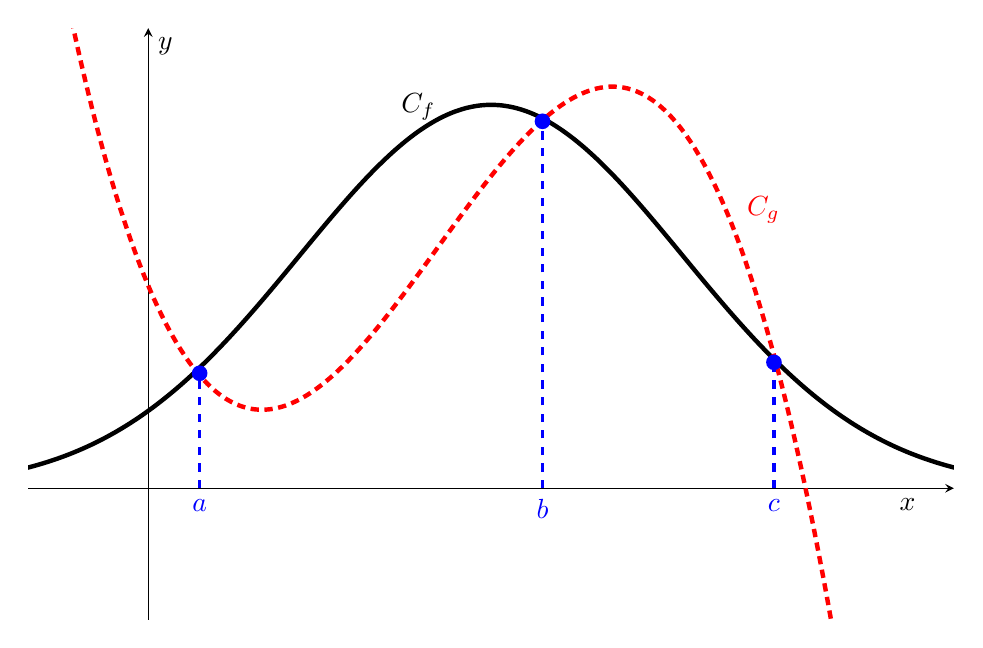
\begin{tikzpicture}[scale=1]
\begin{axis}[
axis x line=bottom,
axis y line = left,
axis lines=middle,
width=1.1*\linewidth,
height=0.75*\linewidth,
xmin=-0.5, xmax=4.5,
ymin=-1, ymax=4,
enlargelimits={abs=0.2},
xlabel={$x$},
ylabel={$y$},
ticks=none,
%ytick distance=1,
%axis equal,
yticklabel=\empty,
xticklabel=\empty,
xlabel style={at={(ticklabel* cs:0.95)},below=0.1},
]
\addplot[samples=101,smooth,ultra thick,domain=(-2:5),mark=none]{3.5*e^(-0.4*(x-2)^2)} node [pos=0.5,above] {$\mathscr C_f$};
\addplot[samples=101,smooth,ultra thick,domain=(-2:5),mark=none,color=red, densely dashed]{-0.69*x^3+3.49*x^2-3.72*x+1.85} node [pos=0.65,above right,color=red] {$\mathscr C_g$};

\addplot +[mark=none,color=blue,style=dashed,very thick] coordinates {(0.3,0) (0.3, 1.05)} node [pos=0,below] {$a$} node[pos=1,circle, minimum size=1pt,fill,inner sep=2pt] {};
\addplot +[mark=none,color=blue,style=dashed,very thick] coordinates {(2.3,0) (2.3, 3.35)} node [pos=0,below] {$b$} node[pos=1,circle, minimum size=1pt,fill,inner sep=2pt] {};
\addplot +[mark=none,color=blue,style=dashed,very thick] coordinates {(3.65,0) (3.65, 1.15)} node [pos=0,below] {$c$} node[pos=1,circle, minimum size=1pt,fill,inner sep=2pt] {};
%\addplot +[mark=none,color=red,style=dashed,very thick] coordinates {(-1, 0) (-1, 2)};
%\addplot +[mark=none,color=red,style=dashed,very thick] coordinates {(-1, 2) (0, 2)};
%\node[label={0:{$(0,1)$}},rectangle,fill,inner sep=2pt] at (axis cs:0,1) {};
%\node[label={[label distance=2pt]-90:{$(0,1)$}},rectangle,fill,inner sep=0pt, minimum height=0pt, minimum width=4pt] at (axis cs:1,1) {};
\end{axis}
\end{tikzpicture}}
&
Résoudre l'équation $f(x)=g(x)$ signifie trouver les nombres qui ont la même image par $f$ et $g$.

Cela revient donc à chercher l'abscisse des points d'intersection des deux courbes $\mathscr C_f$ et $\mathscr C_g$.

Ici, l'ensemble des solution de l'équation est:$$S=\{ a;b;c \}$$
\\ \hline

\end{tabularx}
\end{center}

\begin{exs} \ 
\begin{center}
\vspace{-2mm}
\begin{tabularx}{\linewidth}{|X|X|X|} \hline
\Centering{
\begin{tikzpicture}
\begin{axis}[
styleglobal,
width=0.9*\linewidth,
xmin=-5, xmax= 5,
ymin=-2, ymax=5,
xtick distance=1,
ytick distance=1,
minor x tick num=0,
minor y tick num=0,
%tick label style = {font=\scriptsize},
]
\addplot[styleplot] plot coordinates {(-4,2) (-2,-1) (0,0) (2,3) (4,0.5)} node[pos=0.8,above right] {$\mathscr C_{f_1}$};
\addplot[styleplot,color=blue,densely dashed] plot coordinates {(-4,4) (4,-1)} node[pos=0.75,above right] {$\mathscr C_{f_2}$};
\end{axis}
\end{tikzpicture}}
&
\Centering{
\begin{tikzpicture}
\begin{axis}[
styleglobal,
width=0.9*\linewidth,
xmin=-2, xmax= 8,
ymin=-2, ymax=5,
xtick distance=1,
ytick distance=1,
minor x tick num=0,
minor y tick num=0,
%tick label style = {font=\scriptsize},
]
\addplot[styleplot] plot coordinates {(-1,4) (1,2) (4,1) (6,4) (7,2)} node[pos=0.9,above right] {$\mathscr C_{g_1}$};
\addplot[styleplot,color=blue,densely dashed] plot coordinates {(-1,1) (3,4) (7,1)} node[pos=0.5,above right] {$\mathscr C_{g_2}$};
\end{axis}
\end{tikzpicture}}
&
\Centering{
\begin{tikzpicture}
\begin{axis}[
styleglobal,
width=0.9*\linewidth,
xmin=-7, xmax= 3,
ymin=-5, ymax=2,
xtick distance=1,
ytick distance=1,
minor x tick num=0,
minor y tick num=0,
%tick label style = {font=\scriptsize},
]
\addplot[styleplot] plot coordinates {(-6,1) (-3,-3) (-2,0) (2,-3.5)} node[pos=0.8,above right] {$\mathscr C_{h_1}$};
\addplot[styleplot,color=blue,densely dashed] plot coordinates {(-6,0) (-3,-4) (-1.5,-1) (2,-4.5)} node[pos=0.95,below left] {$\mathscr C_{h_2}$};
\end{axis}
\end{tikzpicture}}
\\ \hline
\Centering{Résoudre $f_1(x)=f_2(x)$:}
\rule[-1cm]{0pt}{1cm}
&
\Centering{Résoudre $g_1(x)=g_2(x)$:}
\rule[-1cm]{0pt}{1cm}
&
\Centering{Résoudre $h_1(x)=h_2(x)$:}
\rule[-1cm]{0pt}{1cm} \\ \hline
\end{tabularx}
\end{center}
\end{exs}}



\newcommand{\\vvc}{
\begin{center}
\begin{tabularx}{\linewidth}{|X|X|X|} \hline
\Centering{$f(x)>k$} & \Centering{$f(x) \leq k$} & \Centering{$f(x)>g(x)$} \\ \hline
\multicolumn{2}{|c|}{
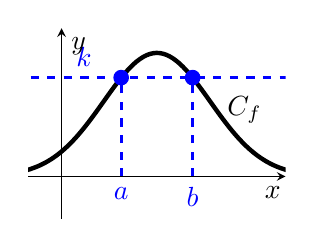
\begin{tikzpicture}[scale=1]
\begin{axis}[
axis x line=bottom,
axis y line = left,
axis lines=middle,
width=0.4*\linewidth,
height=0.33*\linewidth,
xmin=-0.5, xmax=4.5,
ymin=-1, ymax=4,
enlargelimits={abs=0.2},
xlabel={$x$},
ylabel={$y$},
%ytick distance=1,
ticks=none,
grid style=dashed,
%axis equal,
legend pos=north east,
xlabel style={at={(ticklabel* cs:0.95)},below=0.1},
]
\addplot[samples=101,smooth,ultra thick,domain=(-2:5),mark=none]{3.5*e^(-0.4*(x-2)^2)} node [pos=0.75,right] {$\mathscr C_f$};

\addplot +[mark=none,color=blue,style=dashed,very thick] coordinates {(-1,2.8) (5, 2.8)} node [pos=0.18,above right] {$k$};
\node[circle, minimum size=1pt,fill,color=blue,inner sep=2pt] at (axis cs:1.25,2.8) {};
\node[circle, minimum size=1pt,fill,color=blue,inner sep=2pt] at (axis cs:2.75,2.8) {};
\addplot +[mark=none,color=blue,style=dashed,very thick] coordinates {(1.25,0) (1.25, 2.8)} node [pos=0,below] {$a$};
\addplot +[mark=none,color=blue,style=dashed,very thick] coordinates {(2.75,0) (2.75, 2.8)} node [pos=0,below] {$b$};
%\addplot +[mark=none,color=red,style=dashed,very thick] coordinates {(-1, 0) (-1, 2)};
%\addplot +[mark=none,color=red,style=dashed,very thick] coordinates {(-1, 2) (0, 2)};
%\node[label={0:{$(0,1)$}},rectangle,fill,inner sep=2pt] at (axis cs:0,1) {};
%\node[label={[label distance=2pt]-90:{$(0,1)$}},rectangle,fill,inner sep=0pt, minimum height=0pt, minimum width=4pt] at (axis cs:1,1) {};
\end{axis}
\end{tikzpicture}}
&
\Centering{
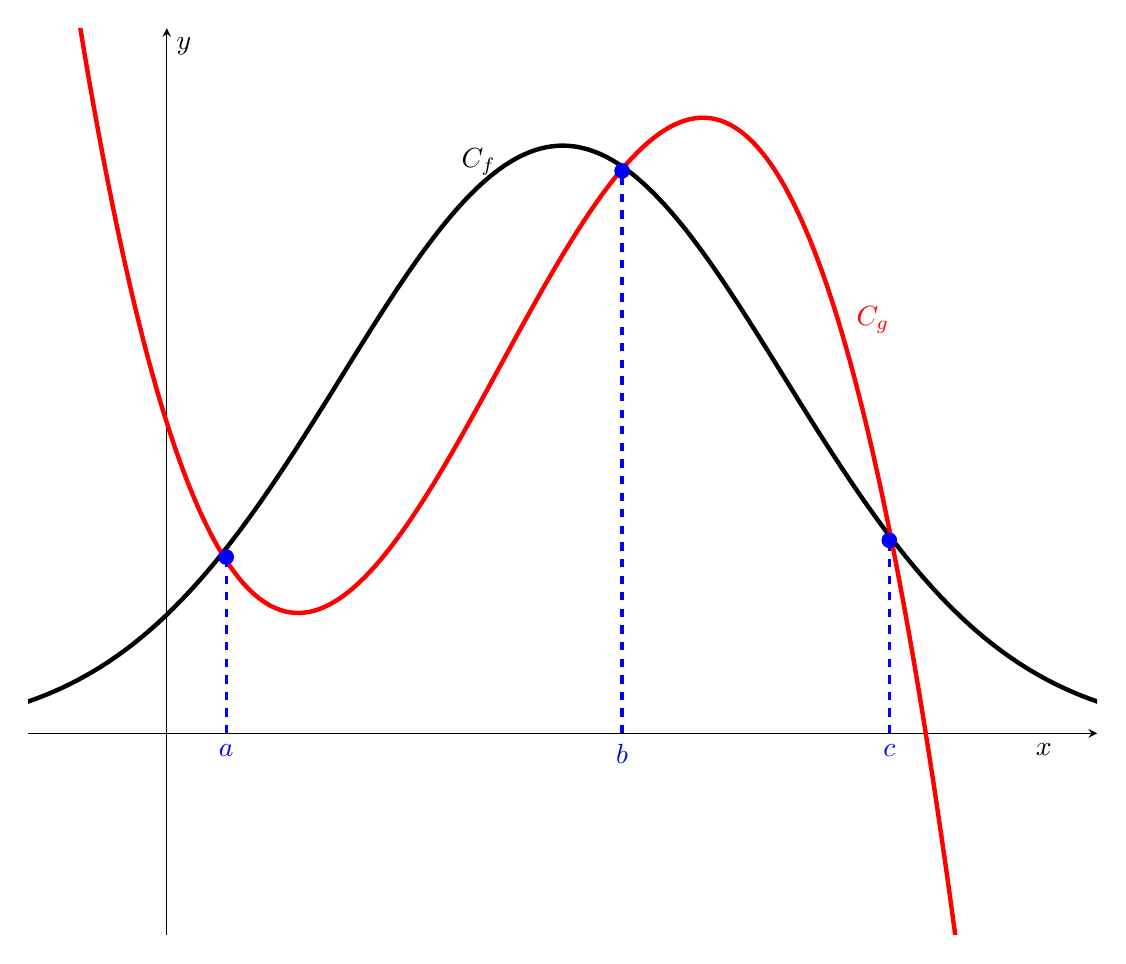
\begin{tikzpicture}[scale=1]
\begin{axis}[
axis x line=bottom,
axis y line = left,
axis lines=middle,
width=1.25*\linewidth,
height=1.08*\linewidth,
xmin=-0.5, xmax=4.5,
ymin=-1, ymax=4,
enlargelimits={abs=0.2},
xlabel={$x$},
ylabel={$y$},
ticks=none,
%ytick distance=1,
%axis equal,
yticklabel=\empty,
xticklabel=\empty,
xlabel style={at={(ticklabel* cs:0.95)},below=0.1},
]
\addplot[samples=101,smooth,ultra thick,domain=(-2:5),mark=none]{3.5*e^(-0.4*(x-2)^2)} node [pos=0.5,above] {$\mathscr C_f$};
\addplot[samples=101,smooth,ultra thick,domain=(-2:5),mark=none,color=red]{-0.69*x^3+3.49*x^2-3.72*x+1.85} node [pos=0.65,above right,color=red] {$\mathscr C_g$};

\addplot +[mark=none,color=blue,style=dashed,very thick] coordinates {(0.3,0) (0.3, 1.05)} node [pos=0,below] {$a$} node[pos=1,circle, minimum size=1pt,fill,inner sep=2pt] {};
\addplot +[mark=none,color=blue,style=dashed,very thick] coordinates {(2.3,0) (2.3, 3.35)} node [pos=0,below] {$b$} node[pos=1,circle, minimum size=1pt,fill,inner sep=2pt] {};
\addplot +[mark=none,color=blue,style=dashed,very thick] coordinates {(3.65,0) (3.65, 1.15)} node [pos=0,below] {$c$} node[pos=1,circle, minimum size=1pt,fill,inner sep=2pt] {};
%\addplot +[mark=none,color=red,style=dashed,very thick] coordinates {(-1, 0) (-1, 2)};
%\addplot +[mark=none,color=red,style=dashed,very thick] coordinates {(-1, 2) (0, 2)};
%\node[label={0:{$(0,1)$}},rectangle,fill,inner sep=2pt] at (axis cs:0,1) {};
%\node[label={[label distance=2pt]-90:{$(0,1)$}},rectangle,fill,inner sep=0pt, minimum height=0pt, minimum width=4pt] at (axis cs:1,1) {};
\end{axis}
\end{tikzpicture}}
\\ \hline
Résoudre l'inéquation $f(x)>k$ signifie trouver les nombres qui ont une image supérieure à $k$.

Cela revient donc à chercher l'abscisse des points de la courbe se situant "au dessus" de la droite d'équation $y=k$.

Ici, l'ensemble des solution de l'inéquation est:$$S=\left] a;b \right[$$ \vspace{-5mm}
&
Résoudre l'inéquation $f(x) \leq k$ signifie trouver les nombres qui ont une image inférieure à $k$.

Cela revient donc à chercher l'abscisse des points de la courbe se situant "en dessous" de la droite d'équation $y=k$.

Ici, l'ensemble des solution de l'inéquation est:$$S=\left] - \infty;a \right] \cup \left[ b ; + \infty \right[$$ \vspace{-5mm}
&
Résoudre l'inéquation $f(x) > g(x)$ signifie trouver les nombres dont l'image par $f$ est supérieure à l'image par $g$.
Cela revient à chercher l'abscisse des points de $\mathscr C_f$ situés "au dessus" des points de $\mathscr C_g$.

Ici, l'ensemble des solutions de l'inéquation est:$$S=\left] - \infty;a \right[ \cup \left] b ; c \right[$$ \vspace{-5mm} \\ \hline
\end{tabularx}
\end{center}
}

\begin{document}

\\vva

\vfill

\\vvb

\renewcommand\tabularxcolumn[1]{p{#1}}
\\vvc

\begin{exs} \ 
\begin{center}
\vspace{-2mm}
\begin{tabularx}{\linewidth}{|X|X|X|} \hline
\Centering{
\begin{tikzpicture}
\begin{axis}[
styleglobal,
width=0.9*\linewidth,
xmin=-5, xmax= 5,
ymin=-2, ymax=5,
xtick distance=1,
ytick distance=1,
minor x tick num=0,
minor y tick num=0,
%tick label style = {font=\scriptsize},
]
\addplot[styleplot] plot coordinates {(-4,2) (-2,-1) (0,0) (2,3) (4,1.5)};
\end{axis}
\end{tikzpicture}}
&
\Centering{
\begin{tikzpicture}
\begin{axis}[
styleglobal,
width=0.9*\linewidth,
xmin=-2, xmax= 8,
ymin=-1, ymax=6,
xtick distance=1,
ytick distance=1,
minor x tick num=0,
minor y tick num=0,
%tick label style = {font=\scriptsize},
]
\addplot[styleplot] plot coordinates {(-1,4) (4,2) (5,4) (7,-1.5)};
\end{axis}
\end{tikzpicture}}
&
\Centering{
\begin{tikzpicture}
\begin{axis}[
styleglobal,
width=0.9*\linewidth,
xmin=-2, xmax= 8,
ymin=-2, ymax=5,
xtick distance=1,
ytick distance=1,
minor x tick num=0,
minor y tick num=0,
%tick label style = {font=\scriptsize},
]
\addplot[styleplot] plot coordinates {(-1,4) (1,2) (4,1) (6,4) (7,2)} node[pos=0.9,above right] {$\mathscr C_{h_1}$};
\addplot[styleplot,color=blue,densely dashed] plot coordinates {(-1,1) (3,4) (7,1)} node[pos=0.5,above right] {$\mathscr C_{h_2}$};
\end{axis}
\end{tikzpicture}}
\\ \hline
\Centering{Résoudre $f(x) \leq 1$:}
\rule[-1cm]{0pt}{1cm}
&
\Centering{Résoudre $g(x)>1$:}
\rule[-1cm]{0pt}{1cm}
&
\Centering{Résoudre $h_1(x) \geq h_2(x)$:}
\rule[-1cm]{0pt}{1cm} \\ \hline
\end{tabularx}
\end{center}
\end{exs}

\end{document}

\begin{comment}
\newpage

\setcounter{section}{2}
\section{ANCIEN - Résolution graphique d'équations et d'inéquations}

\subsection{Equations}

\begin{center}
\begin{tabularx}{\linewidth}{|X|X| } \hline
\Centering{$f(x)=k$} & \Centering{$f(x)=g(x)$} \\ \hline
\Centering{
\begin{tikzpicture}[scale=1]
\begin{axis}[
axis x line=bottom,
axis y line = left,
axis lines=middle,
width=1.2*\linewidth,
height=0.9*\linewidth,
xmin=-0.5, xmax=4.5,
ymin=-1, ymax=4,
enlargelimits={abs=0.2},
xlabel={$x$},
ylabel={$y$},
%ytick distance=1,
ticks=none,
grid style=dashed,
%axis equal,
legend pos=north east,
xlabel style={at={(ticklabel* cs:0.95)},below=0.1},
]
\addplot[samples=101,smooth,ultra thick,domain=(-2:5),mark=none]{3.5*e^(-0.4*(x-2)^2)} node [pos=0.75,right] {$\mathscr C_f$};

\addplot +[mark=none,color=blue,style=dashed,very thick] coordinates {(-1,2.8) (5, 2.8)} node [pos=0.18,above right] {$k$};
\node[circle, minimum size=1pt,fill,color=blue,inner sep=2pt] at (axis cs:1.25,2.8) {};
\node[circle, minimum size=1pt,fill,color=blue,inner sep=2pt] at (axis cs:2.75,2.8) {};
\addplot +[mark=none,color=blue,style=dashed,very thick] coordinates {(1.25,0) (1.25, 2.8)} node [pos=0,below] {$x_1$};
\addplot +[mark=none,color=blue,style=dashed,very thick] coordinates {(2.75,0) (2.75, 2.8)} node [pos=0,below] {$x_2$};
%\addplot +[mark=none,color=red,style=dashed,very thick] coordinates {(-1, 0) (-1, 2)};
%\addplot +[mark=none,color=red,style=dashed,very thick] coordinates {(-1, 2) (0, 2)};
%\node[label={0:{$(0,1)$}},rectangle,fill,inner sep=2pt] at (axis cs:0,1) {};
%\node[label={[label distance=2pt]-90:{$(0,1)$}},rectangle,fill,inner sep=0pt, minimum height=0pt, minimum width=4pt] at (axis cs:1,1) {};
\end{axis}
\end{tikzpicture}}
&
\Centering{
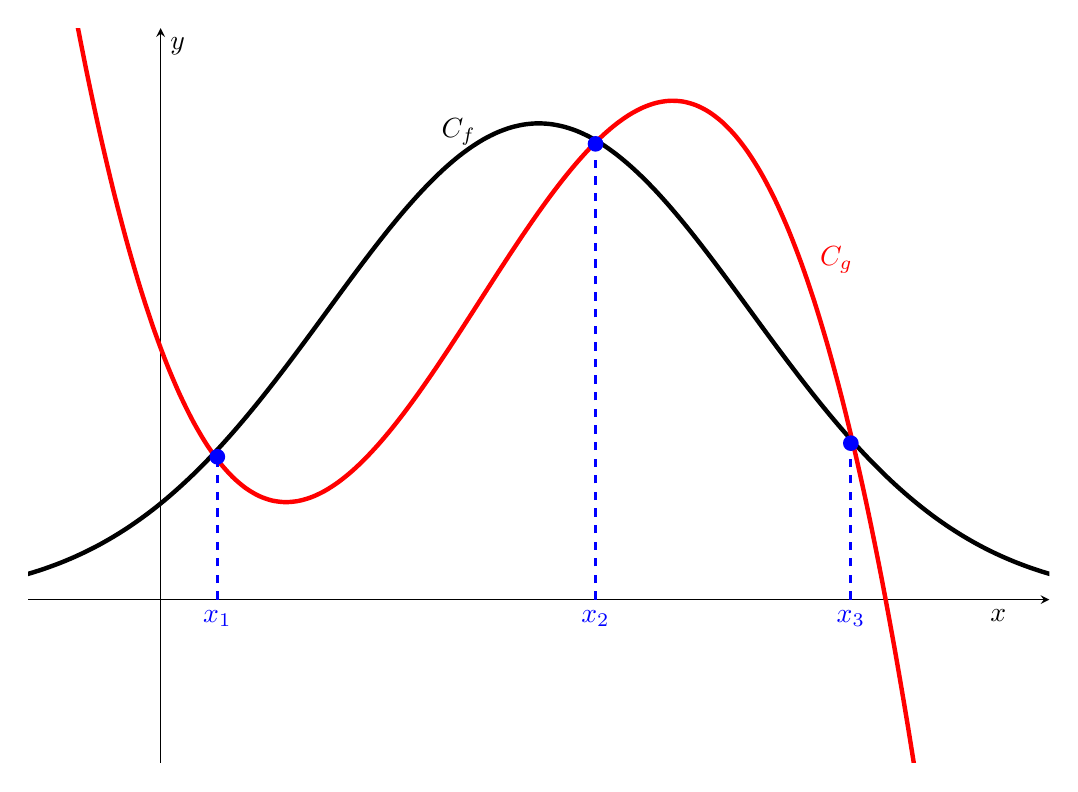
\begin{tikzpicture}[scale=1]
\begin{axis}[
axis x line=bottom,
axis y line = left,
axis lines=middle,
width=1.2*\linewidth,
height=0.9*\linewidth,
xmin=-0.5, xmax=4.5,
ymin=-1, ymax=4,
enlargelimits={abs=0.2},
xlabel={$x$},
ylabel={$y$},
ticks=none,
%ytick distance=1,
%axis equal,
yticklabel=\empty,
xticklabel=\empty,
xlabel style={at={(ticklabel* cs:0.95)},below=0.1},
]
\addplot[samples=101,smooth,ultra thick,domain=(-2:5),mark=none]{3.5*e^(-0.4*(x-2)^2)} node [pos=0.5,above] {$\mathscr C_f$};
\addplot[samples=101,smooth,ultra thick,domain=(-2:5),mark=none,color=red]{-0.69*x^3+3.49*x^2-3.72*x+1.85} node [pos=0.65,above right,color=red] {$\mathscr C_g$};

\addplot +[mark=none,color=blue,style=dashed,very thick] coordinates {(0.3,0) (0.3, 1.05)} node [pos=0,below] {$x_1$} node[pos=1,circle, minimum size=1pt,fill,inner sep=2pt] {};
\addplot +[mark=none,color=blue,style=dashed,very thick] coordinates {(2.3,0) (2.3, 3.35)} node [pos=0,below] {$x_2$} node[pos=1,circle, minimum size=1pt,fill,inner sep=2pt] {};
\addplot +[mark=none,color=blue,style=dashed,very thick] coordinates {(3.65,0) (3.65, 1.15)} node [pos=0,below] {$x_3$} node[pos=1,circle, minimum size=1pt,fill,inner sep=2pt] {};
%\addplot +[mark=none,color=red,style=dashed,very thick] coordinates {(-1, 0) (-1, 2)};
%\addplot +[mark=none,color=red,style=dashed,very thick] coordinates {(-1, 2) (0, 2)};
%\node[label={0:{$(0,1)$}},rectangle,fill,inner sep=2pt] at (axis cs:0,1) {};
%\node[label={[label distance=2pt]-90:{$(0,1)$}},rectangle,fill,inner sep=0pt, minimum height=0pt, minimum width=4pt] at (axis cs:1,1) {};
\end{axis}
\end{tikzpicture}}
\\ \hline
Résoudre l'équation $f(x)=k$ signifie trouver les antécédents de $k$ par la fonction $f$.

Cela revient donc à chercher l'abscisse des points d'intersection de la courbe avec la droite d'équation $y=k$.

Ici, l'ensemble des solution de l'équation est:$$S=\{x_1;x_2 \}$$ \vspace{-5mm}
&
Résoudre l'équation $f(x)=k$ signifie trouver les nombres qui ont la même image par $f$ et $g$.

Cela revient donc à chercher l'abscisse des points d'intersection des deux courbes $\mathscr C_f$ et $\mathscr C_g$.

Ici, l'ensemble des solution de l'équation est:$$S=\{x_1;x_2;x_3 \}$$ \vspace{-5mm}\\ \hline
\end{tabularx}
\vfill
\subsection{Inéquations}

\begin{tabularx}{\linewidth}{ |X|X|X| } \hline
\Centering{$f(x)>k$} & \Centering{$f(x) \leq k$} & \Centering{$f(x)>g(x)$} \\ \hline
\multicolumn{2}{|c|}{
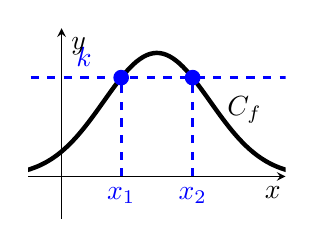
\begin{tikzpicture}[scale=1]
\begin{axis}[
axis x line=bottom,
axis y line = left,
axis lines=middle,
width=0.4*\linewidth,
height=0.33*\linewidth,
xmin=-0.5, xmax=4.5,
ymin=-1, ymax=4,
enlargelimits={abs=0.2},
xlabel={$x$},
ylabel={$y$},
%ytick distance=1,
ticks=none,
grid style=dashed,
%axis equal,
legend pos=north east,
xlabel style={at={(ticklabel* cs:0.95)},below=0.1},
]
\addplot[samples=101,smooth,ultra thick,domain=(-2:5),mark=none]{3.5*e^(-0.4*(x-2)^2)} node [pos=0.75,right] {$\mathscr C_f$};

\addplot +[mark=none,color=blue,style=dashed,very thick] coordinates {(-1,2.8) (5, 2.8)} node [pos=0.18,above right] {$k$};
\node[circle, minimum size=1pt,fill,color=blue,inner sep=2pt] at (axis cs:1.25,2.8) {};
\node[circle, minimum size=1pt,fill,color=blue,inner sep=2pt] at (axis cs:2.75,2.8) {};
\addplot +[mark=none,color=blue,style=dashed,very thick] coordinates {(1.25,0) (1.25, 2.8)} node [pos=0,below] {$x_1$};
\addplot +[mark=none,color=blue,style=dashed,very thick] coordinates {(2.75,0) (2.75, 2.8)} node [pos=0,below] {$x_2$};
%\addplot +[mark=none,color=red,style=dashed,very thick] coordinates {(-1, 0) (-1, 2)};
%\addplot +[mark=none,color=red,style=dashed,very thick] coordinates {(-1, 2) (0, 2)};
%\node[label={0:{$(0,1)$}},rectangle,fill,inner sep=2pt] at (axis cs:0,1) {};
%\node[label={[label distance=2pt]-90:{$(0,1)$}},rectangle,fill,inner sep=0pt, minimum height=0pt, minimum width=4pt] at (axis cs:1,1) {};
\end{axis}
\end{tikzpicture}}
&
\Centering{
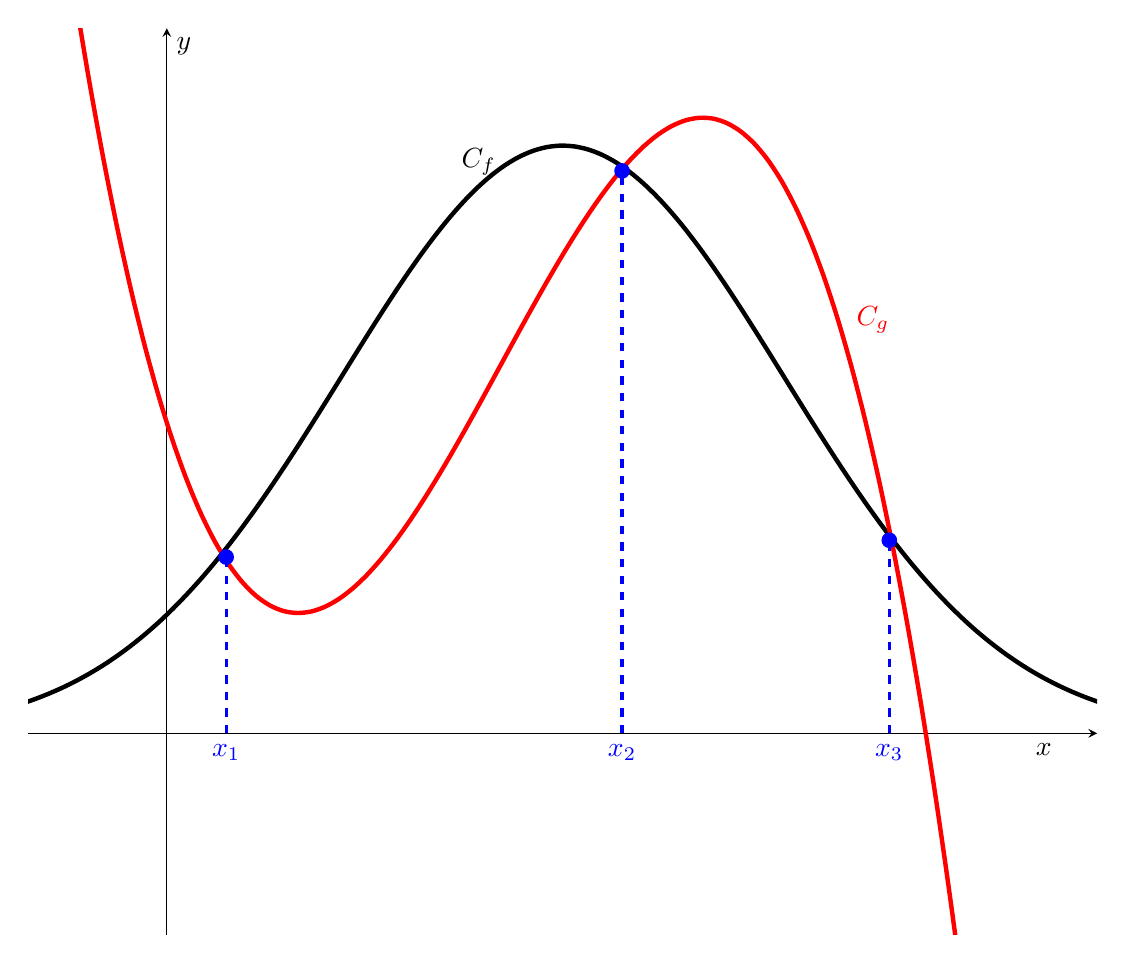
\begin{tikzpicture}[scale=1]
\begin{axis}[
axis x line=bottom,
axis y line = left,
axis lines=middle,
width=1.25*\linewidth,
height=1.08*\linewidth,
xmin=-0.5, xmax=4.5,
ymin=-1, ymax=4,
enlargelimits={abs=0.2},
xlabel={$x$},
ylabel={$y$},
ticks=none,
%ytick distance=1,
%axis equal,
yticklabel=\empty,
xticklabel=\empty,
xlabel style={at={(ticklabel* cs:0.95)},below=0.1},
]
\addplot[samples=101,smooth,ultra thick,domain=(-2:5),mark=none]{3.5*e^(-0.4*(x-2)^2)} node [pos=0.5,above] {$\mathscr C_f$};
\addplot[samples=101,smooth,ultra thick,domain=(-2:5),mark=none,color=red]{-0.69*x^3+3.49*x^2-3.72*x+1.85} node [pos=0.65,above right,color=red] {$\mathscr C_g$};

\addplot +[mark=none,color=blue,style=dashed,very thick] coordinates {(0.3,0) (0.3, 1.05)} node [pos=0,below] {$x_1$} node[pos=1,circle, minimum size=1pt,fill,inner sep=2pt] {};
\addplot +[mark=none,color=blue,style=dashed,very thick] coordinates {(2.3,0) (2.3, 3.35)} node [pos=0,below] {$x_2$} node[pos=1,circle, minimum size=1pt,fill,inner sep=2pt] {};
\addplot +[mark=none,color=blue,style=dashed,very thick] coordinates {(3.65,0) (3.65, 1.15)} node [pos=0,below] {$x_3$} node[pos=1,circle, minimum size=1pt,fill,inner sep=2pt] {};
%\addplot +[mark=none,color=red,style=dashed,very thick] coordinates {(-1, 0) (-1, 2)};
%\addplot +[mark=none,color=red,style=dashed,very thick] coordinates {(-1, 2) (0, 2)};
%\node[label={0:{$(0,1)$}},rectangle,fill,inner sep=2pt] at (axis cs:0,1) {};
%\node[label={[label distance=2pt]-90:{$(0,1)$}},rectangle,fill,inner sep=0pt, minimum height=0pt, minimum width=4pt] at (axis cs:1,1) {};
\end{axis}
\end{tikzpicture}}
\\ \hline
Résoudre l'équation $f(x)>k$ signifie trouver les nombres qui ont une image supérieure à $k$.

Cela revient donc à chercher l'abscisse des points de la courbe se situant "au dessus" de la droite d'équation $y=k$.

Ici, l'ensemble des solution de l'équation est:$$S=\left] x_1;x_2 \right[$$ \vspace{-5mm}
&
Résoudre l'équation $f(x)<k$ signifie trouver les nombres qui ont une image inférieure à $k$.

Cela revient donc à chercher l'abscisse des points de la courbe se situant "en dessous" de la droite d'équation $y=k$.

Ici, l'ensemble des solution de l'équation est:$$S=\left] - \infty;x_1 \right] \cup \left[ x_2 ; + \infty \right[$$ \vspace{-5mm}
&
Résoudre l'inéquation $f(x) > g(x)$ signifie trouver les nombres dont l'image par $f$ est supérieure à l'image par $g$.

Cela revient à chercher l'abscisse des points de $\mathscr C_f$ situés "au dessus" des points de $\mathscr C_g$. \vspace{-5mm} \\ \hline
\end{tabularx}
\end{center}
\end{comment}

\end{document}
